\documentclass[a4paper]{ctexart}
\usepackage[utf8]{inputenc}
\usepackage[a4paper]{geometry}
\usepackage{graphicx}
\usepackage{float}
\usepackage{hyperref}
\usepackage[heading = false]{ctex}
\usepackage{xcolor}
\usepackage{fontspec}
\usepackage{listings}
\usepackage{color}
\pagestyle{plain}
\geometry{top=1.0cm, bottom=2.0cm}

\definecolor{dkgreen}{rgb}{0,0.6,0}
\definecolor{gray}{rgb}{0.5,0.5,0.5}
\definecolor{mauve}{rgb}{0.58,0,0.82}

\lstset{
  frame=tb,
  aboveskip=3mm,
  belowskip=3mm,
  showstringspaces=false,
  columns=flexible,
  basicstyle={\small\ttfamily},
  numbers=none,
  numberstyle=\tiny\color{gray},
  keywordstyle=\color{blue},
  commentstyle=\color{dkgreen},
  stringstyle=\color{mauve},
  breaklines=true,
  breakatwhitespace=true,
  tabsize=3
}
\lstset{
    basicstyle = \ttfamily,
    commentstyle = \itshape,
    numberstyle = \zihao{-5}\ttfamily,
}

\begin{document}
  \begin{titlepage}
      \songti
      \begin{center}
        \vspace*{2cm}
        
\includegraphics[width=0.7\textwidth]{../HDU.png}\\
        \vspace*{1cm}
        {\fontsize{36pt}{0}
          \textbf{机器学习实验\\报\quad 告\\}
        }
        \vspace*{12cm}
        {\fontsize{18pt}{0}
          \makebox[80pt]{\textbf{实验名称}} \underline{\makebox[250pt]{\Large 监督学习之分类学习二}}\\
          \vspace*{0.5cm}
          \makebox[80pt]{\textbf{学\qquad 院}} \underline{\makebox[250pt]{\Large 通信工程学院}}\\
          \vspace*{0.5cm}
          \makebox[80pt]{\textbf{专\qquad 业}} \underline{\makebox[250pt]{\Large xxxx}}\\
          \vspace*{0.5cm}
          \makebox[80pt]{\textbf{学\qquad 号}} \underline{\makebox[250pt]{\Large xxxx}}\\
          \vspace*{0.5cm}
          \makebox[80pt]{\textbf{学生姓名}} \underline{\makebox[250pt]{\Large xxx}}\\
        }
      \end{center}
  \end{titlepage}

  \CTEXsetup[format={\Large\bfseries}]{section}

  \newpage
  \section{实验目的}
  \begin{enumerate}
    \item 理解监督学习的目标
    \item 理解分类学习几种基本算法
    \item 掌握Sklearn提供的分类函数k近邻、朴素贝叶斯、支持向量机、决策树、神经网络模型等
  \end{enumerate}

  \section{实验内容与要求}
  \begin{itemize}
    \item \textbf{上证指数涨跌预测}

    \textbf{数据介绍}  网易财经上获得的上证指数的历史数据,爬取了20年的上证指数数据
    \item \textbf{实验目的:} 根据给出的某时间段150天的历史数据,预测当天上证指数的涨跌
    \item \textbf{技术路线:} \verb|sklearn.svm.SVC|

  \end{itemize}

  \section{实验程序与结果}
  \subsection{程序代码}
  \lstinputlisting[language=Python]{lab4.py}
  \subsection{运行结果}
  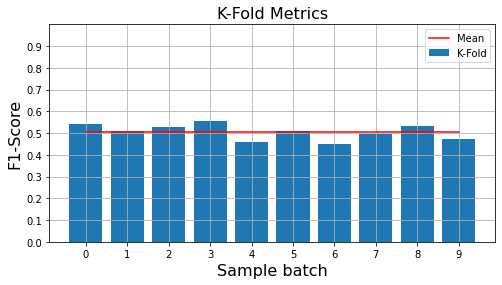
\includegraphics[width=0.7\textwidth]{fig/output.png}

  \section{实验结果分析}
  本次实验选择了数据集中的开盘价、前收盘价、总市值和流通市值作为特征来预测涨跌情况。
  因为数据量较少,因此采用了随机K折交叉验证的方法对样本进行了交叉训练和验证。
  从结果中可以看出,F1-Score平均在0.5左右,说明模型预测的准确率并不高,
  但是也能在一定程度上进行预测。

  \newpage
  \paragraph*{有两个原因可能会导致这种结果}
  \begin{enumerate}
    \item 样本特征的选择与结果相关性差,模型无法从数据中学习到特征
    \item 数据集较少,不足以反映出数据的特征
  \end{enumerate}

  \section{实验问题解答与体会}
  这次实验使用了支持向量机作为训练模型,让我熟悉了支持向量机的相关操作。
  但是这次实验也让我明白机器学习并不总是能够起作用,
  而是要有适当的数据集才能有效的使用机器学习算法。
\end{document}
